%
\chapter{Line of sight velocity variance}
%
\section{Introduction}
%
We will compute in this section the line of sight velocity dispersion of
galaxies in a general spherical density profile, and then compute it
specifically for an NFW profile.

This useful to make cuts at some sigma in the velocity profile to check where
is the most important part of a group.
%
\section{Calculus}
%
By definition, the variance is the mean of the squared quantity under the
assumption of a distribution function. We use a general density profile which
is invariant under rotations $\nu{(r)}$. In our case, we make this mean on the
line of sight, so:
%
\begin{equation}
    \sigma_{LOS}^2\pg{R}\pd=\cfrac{\int_{-\infty}^{\infty}{v_{LOS}^2}\nu{(r)}\dd{z}}
    {\int_{-\infty}^{\infty}\nu{(r)}\dd{z}}
\end{equation}
%
But in the group $r^2=R^2+z^2$ so:
%
\begin{equation}
    \sigma_{LOS}^2\pg{R}\pd=\cfrac{2\int_{R}^{r_{\max}}{v_{LOS}^2}\cfrac{\nu{(r)}{r}}{\sqrt{r^2-R^2}}\dd{r}}
    {2\int_{R}^{r_{\max}}\cfrac{\nu{(r)}{r}}{\sqrt{r^2-R^2}}\dd{r}}
\end{equation}
%
The denominator is by definition the projected density surface along the line
of sight and we denote it
%
\begin{equation}
    \Sigma(R) = 2\int_{R}^{r_{\max}}\cfrac{\nu{(r)}{r}}{\sqrt{r^2-R^2}}\dd{r}
\end{equation}
%
Normally the integration is for $r_{\max}\rightarrow\infty$ but in our
case we want to restrict to a limited region in the group (to virial sphere
precisely).

In the same coordinate system as previously, the line of sight velocity can be
expressed in spherical coordinates as:
%
\begin{equation}
    v_{\mathrm{LOS}} = v_r \cos\theta - v_\theta \sin\theta
\end{equation}
%
We suppose that we are at the equilibrium and so that there is no flow in the
group in consequence we can neglect means of velocities. In terms of velocity
variance we have now:
%
\begin{equation}
    \mysigma\mysiglos = 2\int_R^{r_{\max}}
    \pg{\sigma_r^2(r)\cos^2\theta+\sigma_\theta^2\sin^2\theta}\pd
    \cfrac{\nu{(r)}{r}}{\sqrt{r^2-R^2}}\dd{r}
\end{equation}
%
If we want to use the anisotropy parameter
$\mybeta=1-\sigma_\theta^2(r)/\sigma_r^2(r)$ in case of sphericity\postit{Check
word sphericity!}{5}, we can write:
%
\begin{equation}
    \mysigma\mysiglos = 2\int_R^{r_{\max}}
    \pg{1-\mybeta\cfrac{R^2}{r^2}}\pd
    \cfrac{\nu{(r)}{\sigma_r^2(r)}{r}}{\sqrt{r^2-R^2}}\dd{r}
\end{equation}

We can compute the radial velocity dispersion using the Jeans equation for a
spherical system at equilibrium.
%
\begin{equation}
    \ddp{\pg\nu(r)\sigma_r^2(r)\pd}{r} + \cfrac{2\mybeta}{r}\pg\nu(r)\sigma_r^2(r)\pd=
    -\nu(r)\cfrac{GM(r)}{r^2}
\end{equation}
%
The solution to this equation is given by:
%
\begin{equation}
    \myprofil\sigma_r^2(r)=\int_r^{r_{\max}}K_r(r,s)\nu(s)\cfrac{GM(s)}{s^2}\dd{s}
\end{equation}
%
with $K_r(r,s)$ the kernel of the integral defined as:
%
\begin{equation}
    K_r(r,s)=\exp\left[2\int_r^s\mybeta\cfrac{\dd{t}}{t}\right]
\end{equation}
%
\begin{figure}[H]
    \centering
    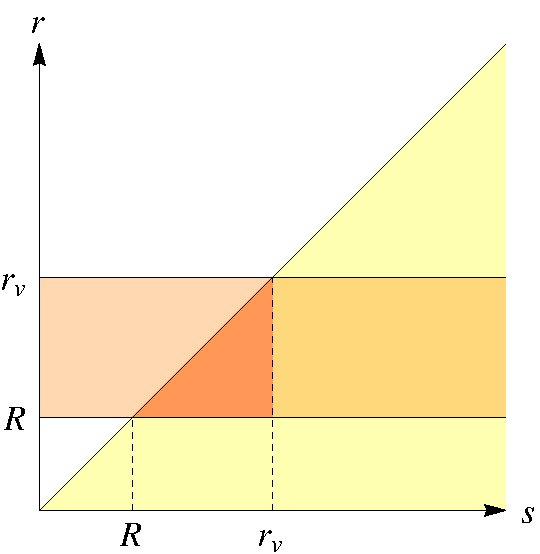
\includegraphics[width=0.5\linewidth]{domint}
    \caption{\footnotesize{}Integration domain for the line of sight radial dispersion.}
\label{fig:domint}
\end{figure}
%
\subsection{Supposing \citet{ML05} anisotropy}
%
With the decomposition of the integral over the domain of integration, we can
write
%
\begin{eqnarray}
    &&\Sigma{(R)}{\sigma_{LOS}}^2{(R)}=2\int_R^{r_v}{\frac{\pg{s+a}\pd}{s^2}{\nu(s)}{G}{M(s)}}{\dd{s}}\nonumber\\
    &\times&\pg\int_R^s{\pg\frac{r}{r+a}-\undemi\pg\frac{R}{r+a}\pd^2\pd\frac{1}{\sqrt{r^2-R^2}}\dd{r}}\pd\nonumber\\
    &+&2\int_{r_v}^{\infty}{\frac{\pg{s+a}\pd}{s^2}{\nu(s)}{G}{M(s)}}{\dd{s}}\nonumber\\
    &\times&\pg\int_R^{r_v}{\pg\frac{r}{r+a}-\undemi\pg\frac{R}{r+a}\pd^2\pd\frac{1}{\sqrt{r^2-R^2}}\dd{r}}\pd\nonumber\\
\end{eqnarray}
%
where we are setting $r_{\max}$ to $r_v$. So now we can write using the
fact that $4a\nu(a)\widetilde{\Sigma}(R/a,c)$:
%
\begin{eqnarray}
    &&{\sigma_{LOS}}^2{(R)}={v_v}^2\frac{c/2}{\widetilde{M}{(c)}\widetilde{\Sigma}{(R/a,c)}}\nonumber\\
    &\times&\pg\int_{R/a}^c{{K}\pg{x\frac{a}{R},\frac{a}{R}}\pd}\widetilde{\nu}{(x)}
    \frac{\widetilde{M}{(x)}}{x}\dd{x}+I\pg{c\frac{a}{R},\frac{a}{R}}\pd{J(c)}\pd\nonumber\\
\end{eqnarray}
%
\begin{equation}
    I(u,u_a)=\left\{\begin{array}{lr}
        -u_a{\rm{sign}}(u_a-1)\frac{{u_a}^2-1/2}{|{u_a}^2-1|^{3/2}}{C^{-1}\pg\frac{1+u{u_a}}{u+u_a}\pd}&\\
        \hspace{5em}+{\rm{acosh}}{u}+\frac{1/2}{u_a+u}\frac{\sqrt{u^2-1}}{{u_a}^2-1},&{u_a}\neq1\\
        {\rm{acosh}}{u}-\sqrt{\frac{u-1}{u+1}}\pg\frac{8+7u}{6(1+u)}\pd,&{u_a}=1\\
    \end{array}\right.
\end{equation}
%
with:
%
\begin{equation}
    K(u,u_a)=\pg{1+\frac{u_a}{u}}\pd{I(u,u_a)}
\end{equation}
%
and:
%
\begin{equation}
    C^{-1}(X)=\left\{\begin{array}{lr}
        {\rm{acosh}}{X}&u_a>1\\
        {\rm{acos}}{X}&u_a<1\\
    \end{array}\right.
\end{equation}
%
We have too an other integral:
%
\begin{equation}
    J(y)=\int_y^{\infty}\frac{x+1}{x^2}\widetilde{\nu}{(x)}\widetilde{M}{(x)}\dd{x}
\end{equation}
%
In the case of an NFW profile, this can be expressed in an analytical way:
%
\begin{align*}
    J(y)&=\frac{2}{3{y^2}(1+y)\pg\ln{4}-1\pd^2}\pg{y}\pg-3+y\pg-9+\pi^2\pg1+y\pd\pd\pd\right.\\
    &+3{y^3}\ln\pg1+\frac{1}{y}\pd+3\ln\pg1+y\pd\pg1-y+y^2\pg1+y\pd\ln\pg1+y\pd\pd\\
    &\left.-3{y^2}\ln\pg{y}\pg1+y\pd\pd+6{y^2}\pg1+y\pd{\dilog{-y}}\pd\\
\end{align*}
%
where the dilogarithm function is defined in our case as:
%
\begin{equation}
    \dilog{z}=-\int_0^1\cfrac{\ln{(1-zt)}}{z}\dd{t}
\end{equation}

Still in the case of the NFW profil, in \citet{MBM10} there is the expression
of $\widetilde{\Sigma}$:
%
\begin{multline}
    \widetilde{\Sigma}(X,c)=\cfrac{1}{2\ln2-1}\int_X^c\cfrac{\dd{x}}{{(1+x)}^2\sqrt{x^2-X^2}}\\
    =\cfrac{1}{2\ln2-1}\begin{cases}
        \cfrac{1}{{(1-X^2)}^{3/2}}
        \cosh^{-1}\left[\cfrac{c+X^2}{(c+1)X}\right]-
        \cfrac{1}{(c+1)}\cfrac{\sqrt{c^2-X^2}}{1-X^2} &\text{if } 0<X<1 \\
    \cfrac{\sqrt{c^2-1}(c+2)}{3{(c+1)}^2} &\text{if } X=1<c\\
    \cfrac{1}{(c+1)}\cfrac{\sqrt{c^2-X^2}}{X^2-1}-
    \cfrac{1}{{(X^2-1)}^{3/2}}
    \cos^{-1}\left[\cfrac{c+X^2}{(c+1)X}\right] &\text{if } 1<X<c\\
    0 &\text{if } X=0\text{or}X>c
    \end{cases}
\end{multline}
